\documentclass[main.tex]{subfiles}

\begin{document}
\sloppy


\vspace{1.0cm}

\section{Introduzione}\label{sec:Introduzione}
Nel mondo dell'eventistica progettare e programmare in anticipo e virtualmente palchi e show è una pratica sempre più diffusa e viene realizzata attraverso programmi detti \say{Previsualizer}. Solitamente vengono utilizzati software\cite{capture} ad-hoc closed-source e molto costosi, con una resa qualitativa molto elevata. Esistono anche dei software gratuiti, molto spesso già inclusi nei sistemi di controllo luci, sempre closed-source, che però omettono molte funzionalità essenziali ed hanno una resa grafica nettamente inferiore.\newline

Lo scopo del progetto CPGDTF-Importer è quello di realizzare un Previsualizer open-source basato su \say{Unreal Engine}\cite{UnrealEngine}, un importante ed affermato software ed engine grafico per la realizzazione di videogiochi, sviluppato dalla \say{Epic Games}. Unreal Engine (da ora abbreviato con \say{UE}) è gratuito e open-source, ha un rendering visivo fotorealistico e mette a disposizione un sistema di plugin con i quali è possibile integrare l'importazione di file non nativi, automatizzare i processi di creazione di \say{oggetti} utilizzabili all'interno dell'engine, oppure definire il comportamento di questi oggetti stessi. UE dispone di una libreria di plugin sviluppati dalla Epic Games tra cui figura \say{DMXEngine}, che già implementa protocolli standard per la gestione di luci e già detta delle basi per sviluppare un proprio plugin nel medesimo contesto.  
\newline
CPGDTF-Importer è, in particolare, un plugin per l'\say{editor} di UE, ovvero quella sezione che permette la creazione di mondi che, nel nostro caso, consisterebbero in palcoscenici virtuali. Il plugin lavorerà principalmente su 3 livelli:
\begin{itemize}
    \item Importazione di luci (chiamate anche \say{fixture}) da un formato standard (GDTF \cite{GDTF}, spiegato nella sezione \ref{subsec:gdtf}), negli \say{Actor} di UE
    \item Importazione di luci sottoforma di Attori all'interno di mondi e gestione delle loro impostazioni
    \item Simulazione in real-time del comportamento delle fixture il più possibile vicino alla realtà
\end{itemize}

\subsection{Anatomia di una fixture}\label{subsec:fixtureAnatomy}
I fari (Che chiameremo anche \say{luci} o \say{fixture}) utilizzati nel mondo dell'eventistica sono dei macchinari di vario tipo e dimensioni che hanno il compito di generare luce di forme e colori differenti. Le fixture che ci interessano sono quelle utilizzate sia come illuminazione di oggetti (Ad esempio, le luci frontali che illuminano un attore in teatro) che come effettistica (Ovvero le luci che fanno effetti aereografici ai concerti). Storicamente le luci nascono come semplici fari monocolore a cui si potevano applicare a mano dei filtri davanti la sorgente luminosa ed a cui si poteva solamente regolare l'intensità attraverso apparecchiature chiamate \say{dimmer}. Solo a partire dagli anni '90 sono entrate in commercio le prime fixture intelligenti, ovvero con la possibilità di essere controllate da remoto attraverso una console luci sfruttando il protocollo DMX \cite{DMX}. 

\subsubsection{Luci statiche e dinamiche}
Le fixture possono essere classificabili come statiche o dinamiche. Le fixture dette \say{statiche} sono fixture che sono formate da un unico \say{blocco} (Che GDTF chiama \say{geometrie}, mentre Unreal Engine chiama \say{SceneComponents}) e che, fisicamente, non si muovono. Sono quelle più semplici nonché il primo tipo di faro entrato in commercio.
\begin{figure}[H]
    \centering
    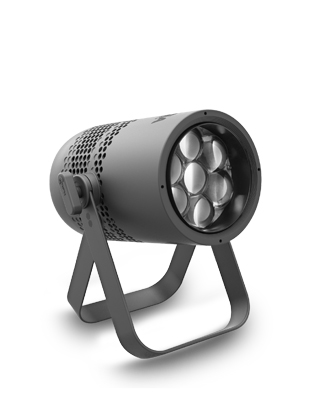
\includegraphics[width=0.4\linewidth]{img/introduzione/staticFixtureExample.jpg}
    \caption{Esempio di fixture statica}
    \label{fig:staticFixture}
\end{figure}
Le fixture dette invece \say{dinamiche} (chiamate anche \say{Teste mobili}) sono composte da più geometrie collegate tra loro da motori, in modo che quella responsabile di emettere il fascio di luce possa roteare, di solito su due assi. Solitamente la geometria che viene poggiata per terra o appesa viene chiamata \say{base}, quella che emette luce \say{testa}
\begin{figure}[H]
    \centering
    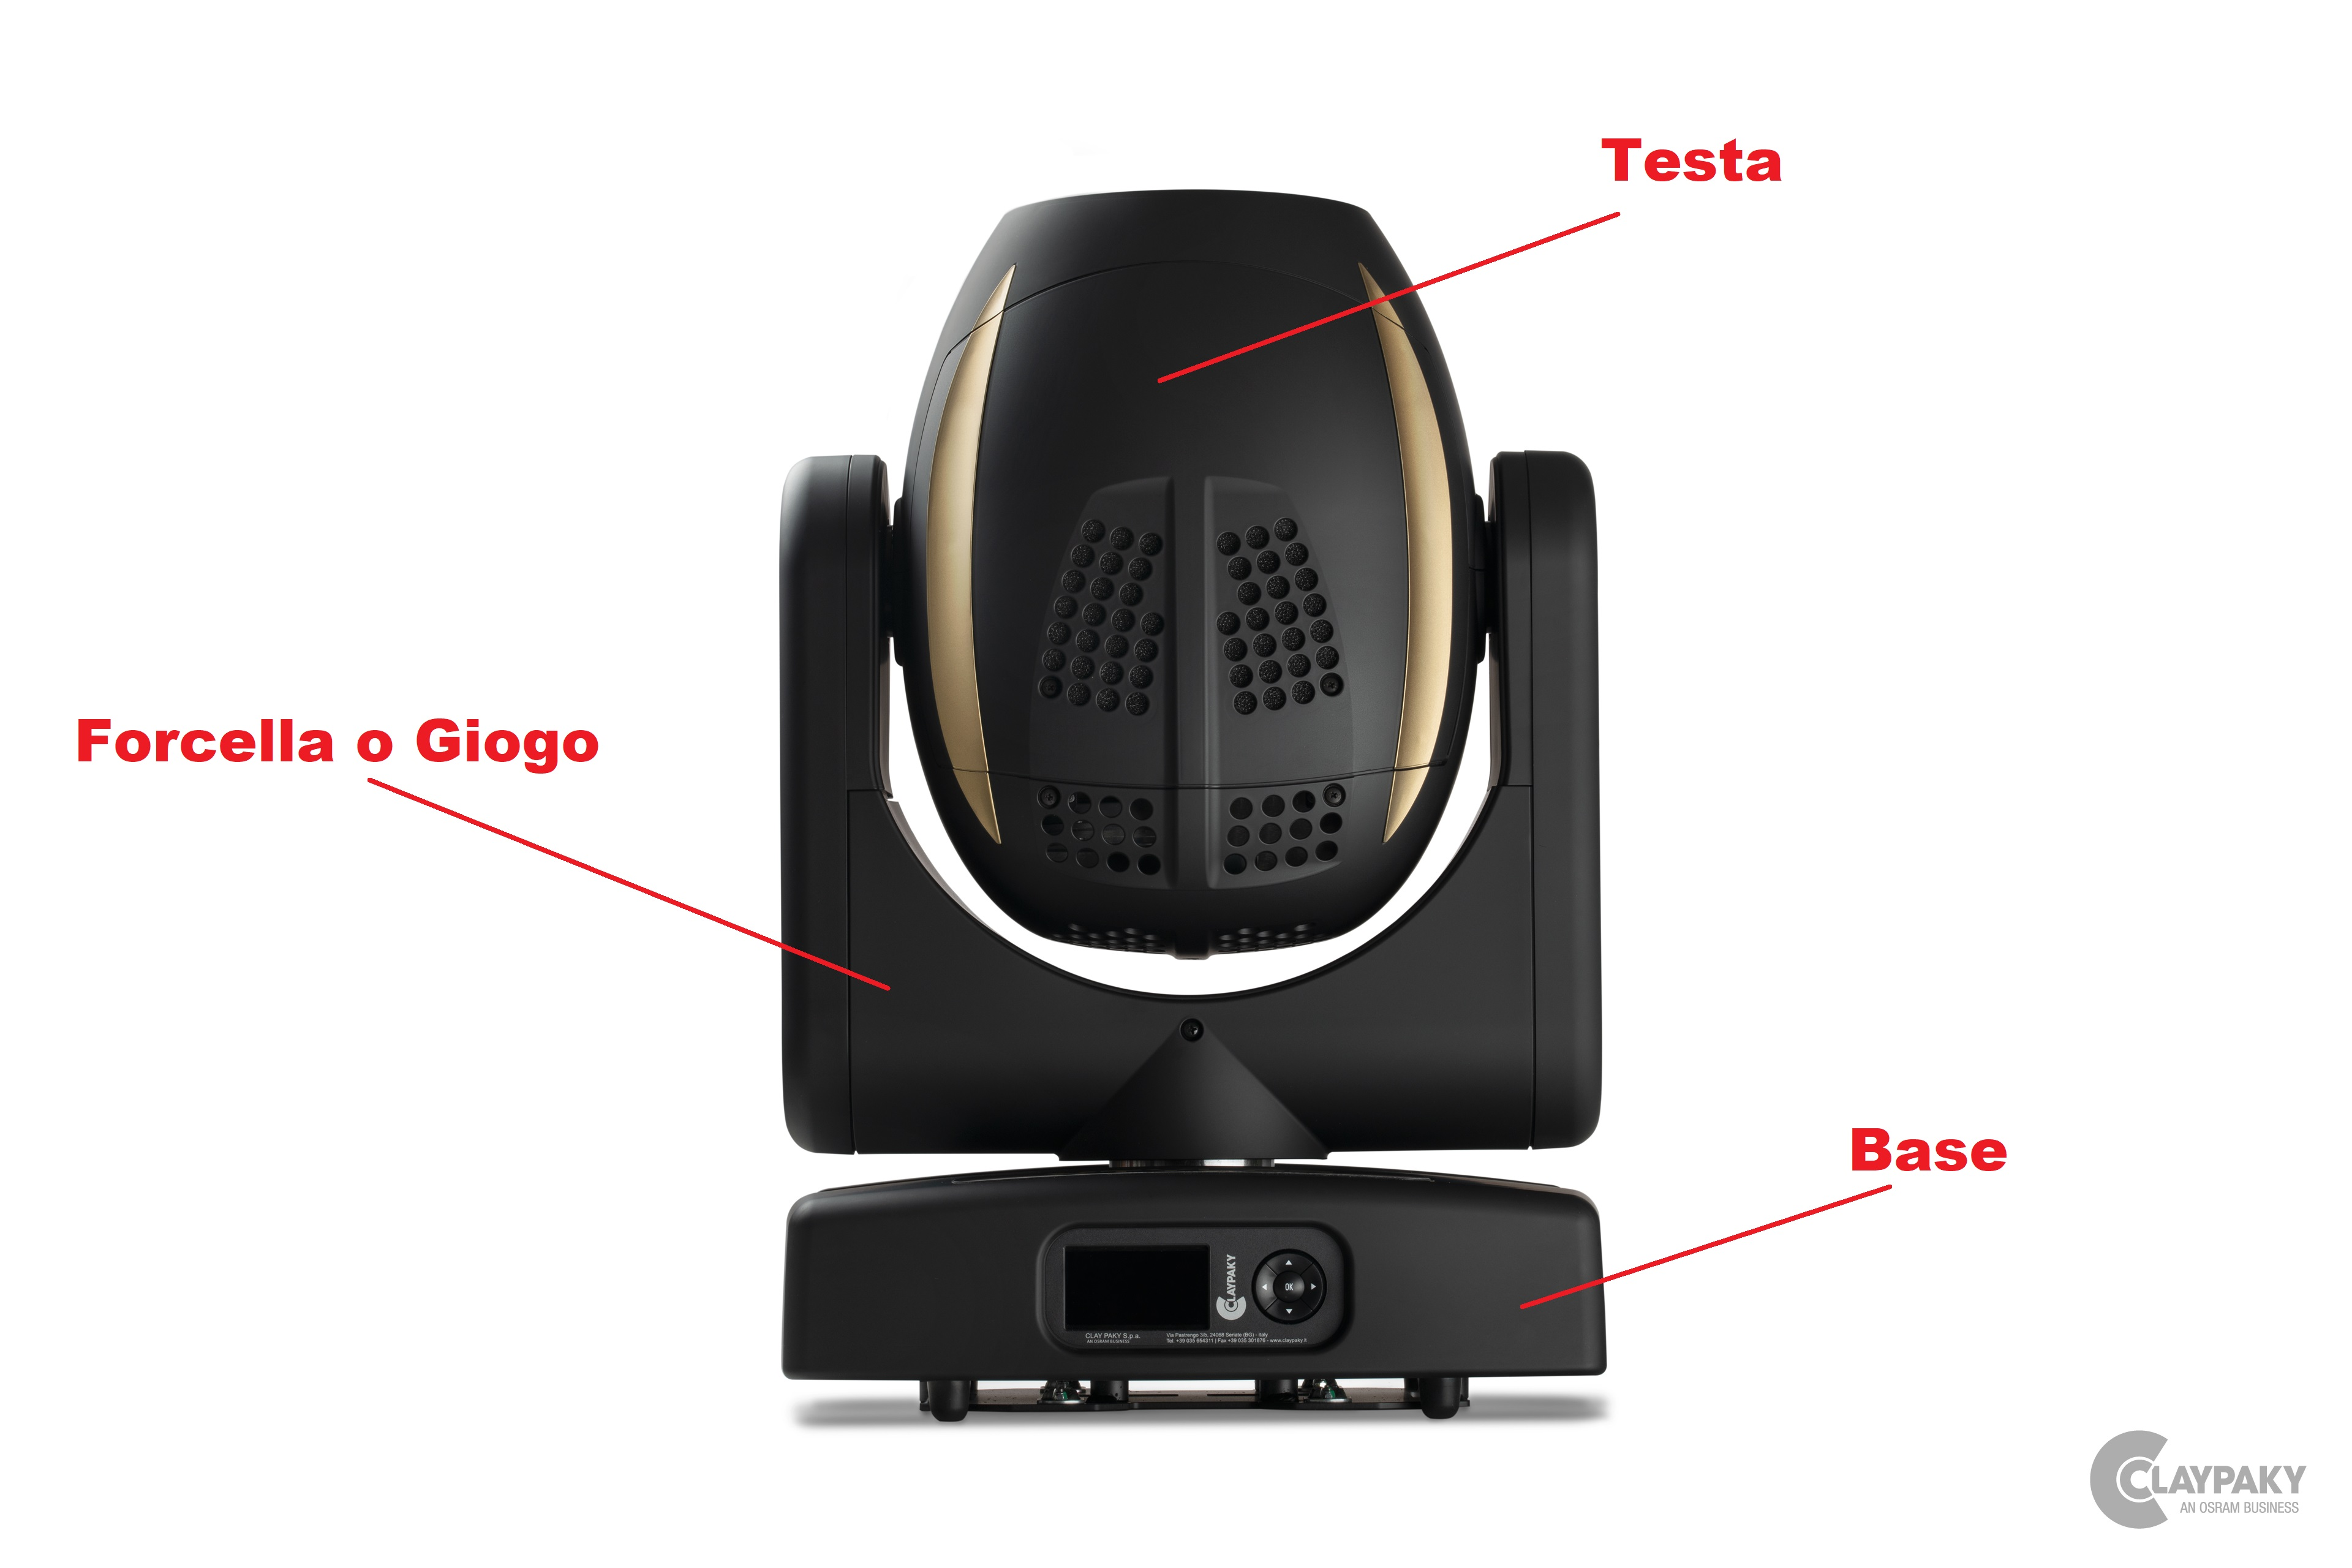
\includegraphics[width=0.75\linewidth]{img/introduzione/dynamicFixtureAnatomy.jpg}
    \caption{Geometrie di un faro dinamico}
    \label{fig:DynamicFixture}
\end{figure}

\subsubsection{Moduli di una luce}
All'interno della testa, così come all'interno delle fixture statiche, è presente una sorgente luminosa che può essere sia bianca se il faro utilizza una sintesi colore sottrattiva, che colorata se il faro utilizza una sintesi colore additiva. La luce viene fatta passare attraverso vari moduli che ne alterano il colore, la messa a fuoco e la forma fino ad uscire dalla lente principale collocata ad una estremità della testa. Su praticamente tutti i fari in commercio non è possibile montare moduli custom o invertirli con quelli di un altro faro. Ciò ci permette di avere un unico file per descrivere interamente il comportamento di un determinato faro. \newline
I moduli che verranno toccati in questo progetto sono i seguenti:
\begin{itemize}
    \item \textbf{Ruote colori e gobo}: Sono delle ruote in cui sopra sono presenti su degli slot, dei filtri colori o delle forme. Hanno sempre uno slot libero in cui la luce può passare senza essere modificata e, girando, possono mettere in mezzo alla luce uno slot alla volta
    \item \textbf{Sintesi e correzione dei colori}: Nelle luci a sintesi additiva troviamo LED di colori differenti (RGB + Bianco, Ambra, Lime, UV, etc); nelle luci a sintesi sottrattiva invece abbiamo una luce bianca e delle flag CMY che vengono inserite davanti per regolarne il colore. Esistono anche dei filtri (sempre sottrattivi) per effettuare una sorta di color correction.
    \item \textbf{Sagomatore}: È un sistema composto da quattro lame che possono essere inserite nel fascio di luce da direzioni differenti e possono essere inclinate, in modo da ritagliare in maniera precisa triangoli e quadrilateri precisi per fare puntamenti.
    \item \textbf{Iris}: Sono delle lame circolari che entrano nel fascio di luce da tutte le direzioni e si occupano di ridurne la dimensione. Il funzionamento è analogo al diaframma di una fotocamera
    \item \textbf{Frost}: È un filtro atto a rendere soffusa la luce, smorzando i bordi di eventuali figure che si stanno proiettando
\end{itemize}
I moduli solitamente funzionano sottrattivamente: per ogni modulo a partire dalla fonte luminosa, andiamo ad occluderla mano a mano per disegnare la forma che vogliamo ottenere.

\subsubsection{Protocollo DMX}
Oggi giorno, quasi tutte le fixture che vengono usate sono intelligenti e, come citato sopra, vengono controllate via DMX. DMX è un protocollo unidirezionale in cui un master (solitamente una console luci) invia 44 volte al secondo agli slave (le varie fixture) un array di 512 byte chiamato \say{Universo DMX}. Le luci hanno memorizzato un offset all'interno di questo array chiamato \say{Indirizzo DMX} che viene impostato manualmente su ognuna dall'operaio che le monta su un palcoscenico. Ogni volta che arriva un nuovo pacchetto DMX la luce inizierà a leggere la sua sezione di dati a partire dall'indirizzo/offset specificato. Ogni byte che legge è chiamato \say{canale} e, solitamente, corrisponde al valore da assegnare ad una diversa funzionalità della luce.
\begin{figure}[H]
    \centering
    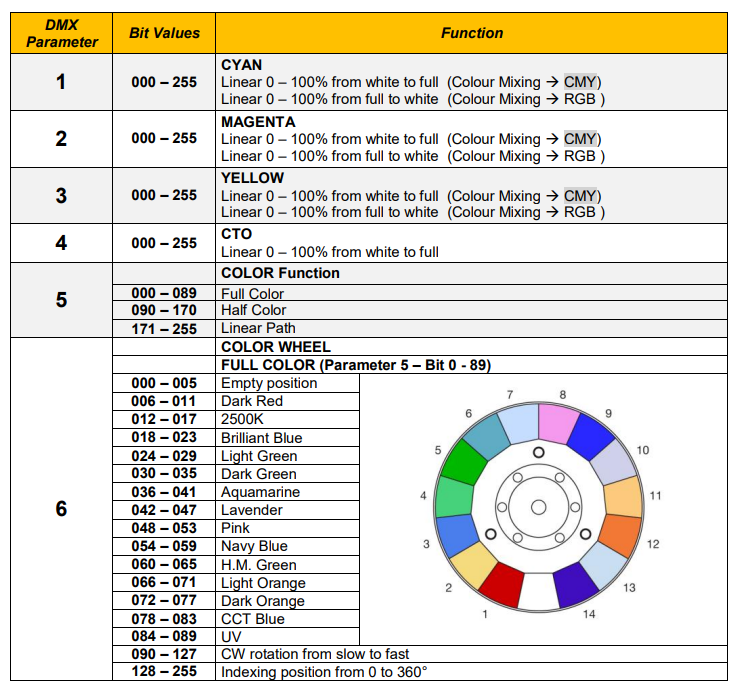
\includegraphics[width=0.65\linewidth]{img/introduzione/dmxChannelDescExample.png}
    \caption{Esempio di canali DMX. Se il canale 1 di questa luce viene portato a FULL (255), la luce si colorerà di azzurro. Se, invece, il canale 6 viene impostato al valore 50, si colorerà di rosa.}
    \label{fig:dmxChannelsExample}
\end{figure}
% TODO FOTO E SCHEMA DEI MODULI IN UNA LUCE APERTA

\subsection{GDTF}\label{subsec:gdtf}
GDTF - \textit{General Device Type Format} - è un formato per descrivere fixture nella maniera più accurata possibile. È stato sviluppato da MAlighting (azienda produttrice del sistema di controllo luci attualmente più usato in show medio-grandi), Robe (altro leader industriale nello sviluppo e realizzazione di luci per l'eventistica) e Vectorworks (Un software di CAD/Deisgn anch'esso molto usato nella progettazione e previsualizzazione di palcoscenici). 
\newline

Un file GDTF è essenzialmente un pacchetto contenente all'interno 

\subsection{Informazioni sul tirocinio}\label{subsec:tirocinio}
CPGDTF-Importer è un progetto sviluppato dalla \say{Clay Paky}, azienda italiana leader mondiale nella progettazione e realizzazione di luci per concerti, architettura e teatri, per cui ho svolto il tirocinio curriculare. Lo sviluppo ha avuto inizio nel Maggio 2022 

\end{document}